% AMOC sensitivity to the 10-m winds in the 2° OMIP ocean: configuration, adjoint, verification, results.
% Figures come from adjoint/plot_fd_scans.jl and adjoint/plot_amoc_sensitivity.jl (configs/plot_*.json).
% Build with `latexmk -pdf omip_amoc_adjoint.tex` in this directory.
\documentclass[11pt]{article}

\usepackage[margin=1in]{geometry}
\usepackage{amsmath, amssymb}
\usepackage{booktabs}
\usepackage{graphicx}
\usepackage{hyperref}
\usepackage{siunitx}
\usepackage{url}
\makeatletter\g@addto@macro\UrlBreaks{\do\_}\makeatother

\newcommand{\vv}{\mathbf{v}}
\newcommand{\uu}{\mathbf{u}}
\newcommand{\xx}{\mathbf{x}}
\newcommand{\gvec}{\mathbf{g}}

\title{\textbf{AMOC sensitivity to the winds in the 2\textdegree{} OMIP ocean}:\\
       configuration, adjoint and verification}
\author{NumericalEarth OMIP adjoint notes (branch \texttt{ajs/omip-adjoint})}
\date{\today}

\begin{document}
\maketitle

\section{Summary}

The package \texttt{OMIPAdjoint} (\path{experiments/OMIPSimulations/adjoint}) computes the gradient of
the Atlantic overturning at \ang{26.5}N with respect to the JRA55 \SI{10}{m} winds that force the
ocean-only 2\textdegree{} OMIP model. The gradient is the Enzyme reverse-mode adjoint of the
Reactant-compiled \textsc{Oceananigans} model. One time step and its reverse pass are compiled once.
The host then drives them on a binomial (Revolve) checkpoint schedule, so the compile cost does not
depend on the window length.

On one A100 (Lonestar6) the gradient runs for windows of 1, 2, 8, 84 (one week) and 360 steps (30 days).
The compile takes \SIrange{27}{29}{min} and the first call about \SI{39}{min}, at every length.
After that a 30-day gradient costs \SI{104}{s}. Finite differences confirm that the adjoint is the exact
local derivative at every length. Past about one day, however, the objective is only piecewise smooth:
it jumps by \SIrange{e-7}{e-3}{Sv} under perturbations of \SIrange{5e-7}{5e-4}{m/s}. That is why
small-step Taylor tests fail there. At finite amplitude (\SIrange{0.25}{1}{m/s}) the gradient predicts
the 30-day response to within \SIrange{0.05}{2}{\percent}. Freezing CATKE's mixing coefficients in the
adjoint (Section~\ref{sec:frozen}) changes the gradient's direction by little (cosine \num{0.994} at 30
days), but it predicts the finite-amplitude response slightly worse than the full adjoint and saves no
time. Its uniform-wind responses can still differ substantially.

\section{Model configuration}

\begin{center}\small
\begin{tabular}{@{}lp{0.72\textwidth}@{}}
\toprule
Item & Setting \\
\midrule
Grid & \textsc{TripolarGrid}, $180\times60\times20$ ($\approx\ang{2}$), halo $(8,8,8)$ \\
Vertical & exponential spacing to \SI{5500}{m} \\
Bathymetry & ETOPO regridded (minimum depth \SI{20}{m}, one major basin, 25 smoothing passes),
             Central American isthmus closed, \texttt{GridFittedBottom} immersed boundary \\
Equations & hydrostatic Boussinesq, \texttt{HydrostaticFreeSurfaceModel}, TEOS-10 \\
Time stepping & split Runge--Kutta 3, $\Delta t = \SI{7200}{s}$ \\
Free surface & split-explicit, 50 substeps (traced as one rolled loop) \\
Momentum advection & WENO, 5th order, explicit in the vertical; enstrophy-conserving Coriolis \\
Tracer advection & WENO, 7th order, explicit in the vertical \\
Vertical closure & CATKE; background diffusivity $\kappa = \max(\num{2e-6}, \num{1e-5}\,|\sin\varphi|)$
                   \si{m^2/s} (Henyey) \\
Lateral closures & GM/Redi, $\kappa_{\text{skew}} = \kappa_{\text{sym}} = \SI{800}{m^2/s}$;
                   biharmonic viscosity with a \SI{50}{day} damping time; implicit bottom drag \\
Atmosphere & JRA55 repeat-year (1990), three-hourly, from 1990-01-01, interpolated onto a regular
             $640\times320$ grid and held in device memory (Float64) \\
Surface fluxes & OMIP-2 Large--Yeager bulk formulae, fixed iteration count; ocean albedo 0.06; no sea ice \\
Initial condition & WOA annual $T, S$ (converted to TEOS-10); ocean at rest \\
Precision / backend & Float64, Reactant 0.2.303 / XLA on one A100 \\
\bottomrule
\end{tabular}
\end{center}

\paragraph{Alternative forcing.} With \texttt{"forcing": "ecco4"} the ocean is a
\texttt{PrescribedFluxOcean} driven by ECCO4's monthly wind stress, net heat flux and net freshwater flux,
from the ECCO4 1993-01 state. The gradient is then with respect to the stress. This configuration has
been verified at 2 steps (Table~\ref{tab:verification}).

\section{The sensitivity problem}

\paragraph{Control.} The control is the \SI{10}{m} wind on every atmosphere cell and forcing slice,
$\uu = (u_{10}, v_{10}) \in \mathbb{R}^{2 \times 640 \times 320 \times S}$, where $S$ is the number of
three-hourly slices covering the window. That is \num{6.6e6} unknowns for 8 steps ($S = 16$) and
\num{1.0e8} for 30 days ($S = 248$). The winds reach the ocean through time interpolation between
slices, regridding to the ocean grid and the bulk formulae. The gradient therefore includes the
dependence of the turbulent heat and freshwater fluxes on the wind, not only the stress.

\paragraph{Forward map.} Each evaluation restores the ocean's prognostic state and every component
clock from a host snapshot. It then recomputes the diagnostic state inside the differentiated window
(interface fluxes first, then the ocean's diagnostics and the stage-1 tendencies) and takes $N$ steps,
$\xx_n = \Phi(\xx_{n-1}; \uu)$, $n = 1,\dots,N$. Recomputing inside the window matters: when the
first step's fluxes were computed outside it, the 1-step gradient was exactly zero.

\paragraph{Objective.} The section is a staircase of cell faces along \ang{26.5}N from \ang{80}W to
\ang{14}W (the RAPID line). In each column it takes the $v$-face nearest the latitude, and it joins
neighboring columns along the $u$-faces between them. It visits tripolar rows 38--40, within
\ang{1.4} of the line. A single grid row would not do: on the tripolar grid it drifts from
\ang{28.4}N to \ang{33.8}N across the Atlantic. Let $W^{v}_{ijk}$ and $W^{u}_{ijk}$ be the signed,
wet-masked face areas, and $a_k$ the section area per level. The transport out of the region south of
the staircase is
\begin{equation}
T_k = \sum_{ij} \left( W^{v}_{ijk}\, v_{ijk} + W^{u}_{ijk}\, u_{ijk} \right).
\end{equation}
The residual streamfunction removes the section-mean normal velocity, so $\psi$ closes at the surface:
\begin{equation}
\tilde T_k = T_k - \frac{\sum_{k'} T_{k'}}{\sum_{k'} a_{k'}}\, a_k, \qquad
\psi_k = -\sum_{k' \le k} \tilde T_{k'} .
\end{equation}
The objective is $\psi$ at the level nearest \SI{1000}{m}, at the end of the window:
\begin{equation}
J(\uu) = 10^{-6}\, \psi_{k_{\text{ref}}}\!\left(\xx_N(\uu)\right) \quad [\si{Sv}].
\label{eq:obj}
\end{equation}
The face weights are precomputed on a CPU twin of the grid. The traced objective is then a pure array
reduction with no element indexing.

\paragraph{Gradient.} Five functions are compiled once: the diagnostic refresh, one coupled time step,
and the reverse passes (\texttt{autodiff(Reverse)}, model \texttt{Duplicated}) of the refresh, the step
and the objective. The host runs them on the Revolve schedule of Griewank and Walther (2000), taken
from \texttt{Checkpointing.jl}. With $c$ checkpoints the forward model is recomputed
$O(\log N)$ times. A checkpoint is a host copy of every device array in the model except the grids and
the forcing. The prognostic snapshot alone is not enough mid-window, because the step computes the
stage-1 tendencies and CATKE's diffusivities before it updates the fluxes. The shadow model carries the
adjoint from one step's reverse pass to the next and accumulates $\gvec = \partial J/\partial \uu$ in
its atmosphere shadows. The compile options keep kernel raising on (\texttt{reshape\_propagate = :none},
\texttt{transpose\_propagate = :up}). They exclude two Reactant rewrite patterns,
\texttt{while\_deadresult} and \texttt{cse\_reduce\_transposed}, which cost tens of minutes on the
differentiated module and change almost nothing.

\paragraph{Frozen mixing.} With \texttt{"frozen\_mixing": true}, the CATKE viscosity and diffusivities
pass through \texttt{ignore\_derivatives} as soon as they are computed. The forward model, and hence
$J$, is unchanged. The adjoint then treats the mixing coefficients as constants: no derivative reaches
the TKE equation or the mixing length.

\section{Verification}

A Taylor test on its own is not enough: it can only show that $\gvec$ is the derivative of the
compiled forward map. Each rung therefore also compares the traced primal with a CPU twin of the same
model. The direction is always $d = \gvec/\lVert\gvec\rVert$, with step sizes $h = 2^{-i}$
\si{m/s}. The verdict fits $\Delta f = a + g h + q h^2$ through the three smallest $h$, so curvature at
large $h$ does not bias the slope.

\begin{table}[h]
\centering\small
\begin{tabular}{@{}p{0.17\textwidth}p{0.11\textwidth}rlp{0.33\textwidth}@{}}
\toprule
Window & Job & $J$ [Sv] & Check & Result \\
\midrule
1 step (rolled) & 3566763 & $-14.3509$ & Taylor & rel.\ err.\ \num{6.1e-5}, second-order remainder \\
1 step, frozen mixing & 3564718 & $-14.3509$ & Taylor vs.\ full FD & \num{1.1e-4}; cosine to full $\gvec$ \num{0.99999968} \\
2 steps (Revolve) & 3565554 & $-28.5631$ & Taylor & \num{2.0e-7}; cosine to unrolled $\gvec$ $1 - \num{4e-10}$ \\
2 steps, ECCO4 & 3566764 & $-34.98$ & Taylor & remainder \num{2.3e-6} of $h\,\gvec^{\mathsf T}d$ at $h = \num{3.1e-3}$ \\
8 steps & 3570013 / 3571322 & $-11.2848$ & FD scan & central difference to \numrange{4e-9}{2e-8} \\
84 steps & 3570014 / 3571323 & $-15.9743$ & FD scan & central to \num{4e-9} for $h \le \num{2.4e-4}$ \\
360 steps & 3570015 / 3571324 & $+16.6320$ & FD scan & forward to \numrange{1e-6}{2e-5} for $h \le \num{3e-5}$ \\
\bottomrule
\end{tabular}
\caption{Verification rungs. The traced primal matches the CPU twin to \num{7.5e-13} (1 step) and
\num{2.2e-15} (2 steps). FD scans evaluate $J$ at $\xx_0 \pm h d$ for 25 octaves of $h$, from \SI{1}{m/s}
down to \SI{6e-8}{m/s}, along the saved gradient. Their $J(\xx_0)$ matches the gradient run's to
\num{4e-14}, \num{2e-11} and \num{4e-12}.}
\label{tab:verification}
\end{table}

$J$ swings in sign over the first month: \num{-14.4}, \num{-28.6}, \num{-11.3}, \num{-16.0} and then
\SI{+16.6}{Sv}. This is the adjustment from rest under the WOA state: Ekman transport, inertial
oscillations (period \SI{27}{h} at \ang{26.5}N) and the barotropic and baroclinic adjustment. It is not
an equilibrium overturning.

\subsection{Longer windows: the objective is piecewise smooth}

Figure~\ref{fig:fd} shows the scans. Beyond one day, small perturbations flip discrete switches in the
forward model. CATKE's convective and stable branches are the likely source, but this is not yet
confirmed. Each flip makes $J$ \emph{jump}: the residual of the linear prediction plateaus over a range
of $h$ instead of falling with it. For example, at 360 steps the $-h$ side is offset by
\SI{-2.6e-7}{Sv} for every $h$ from \num{9.5e-7} to \SI{3e-5}{m/s}. The adjoint differentiates the
branch the forward run took. It therefore agrees with finite differences only inside the smooth
neighborhood around $\xx_0$, and that neighborhood shrinks as the window grows:

\begin{center}\small
\begin{tabular}{@{}rp{0.22\textwidth}p{0.26\textwidth}p{0.3\textwidth}@{}}
\toprule
Steps & Smooth along $\pm d$ & Jumps in $J$ & Central diff.\ vs.\ $\gvec^{\mathsf T}d$, $h = 0.25$--$1$ \\
\midrule
8 & all $h \le 1$ & none & \num{4e-4} \\
84 & $h \le \num{2.4e-4}$ & \SIrange{1e-6}{3e-4}{Sv} for $h \ge \num{4.9e-4}$ & \numrange{5e-3}{7e-3} \\
360 & $+d$: $h \le \num{1.2e-4}$; $-d$: $h \le \num{4.8e-7}$ & \SI{3e-7}{Sv} up to \SI{\sim 1e-3}{Sv} & \num{2e-3} ($h = 0.5$), \num{5e-4} ($h = 0.25$) \\
\bottomrule
\end{tabular}
\end{center}

The earlier Taylor checks at 84 and 360 steps used $h \le \num{1e-2}$ and failed on these jumps, not on
the gradient. At finite amplitude the jumps are small next to $h\,\gvec^{\mathsf T}d$, and the secant
slope matches the adjoint. This holds along $d = \gvec/\lVert\gvec\rVert$, where the signal is largest;
along other directions the same jumps weigh more. Freezing the mixing in the adjoint does not remove the
jumps, because the forward model is unchanged. It changes what $\gvec$ approximates. A frozen-mixing
gradient should therefore be judged by its large-$h$ secants, not by a small-$h$ Taylor test.

\begin{figure}[h]
\centering
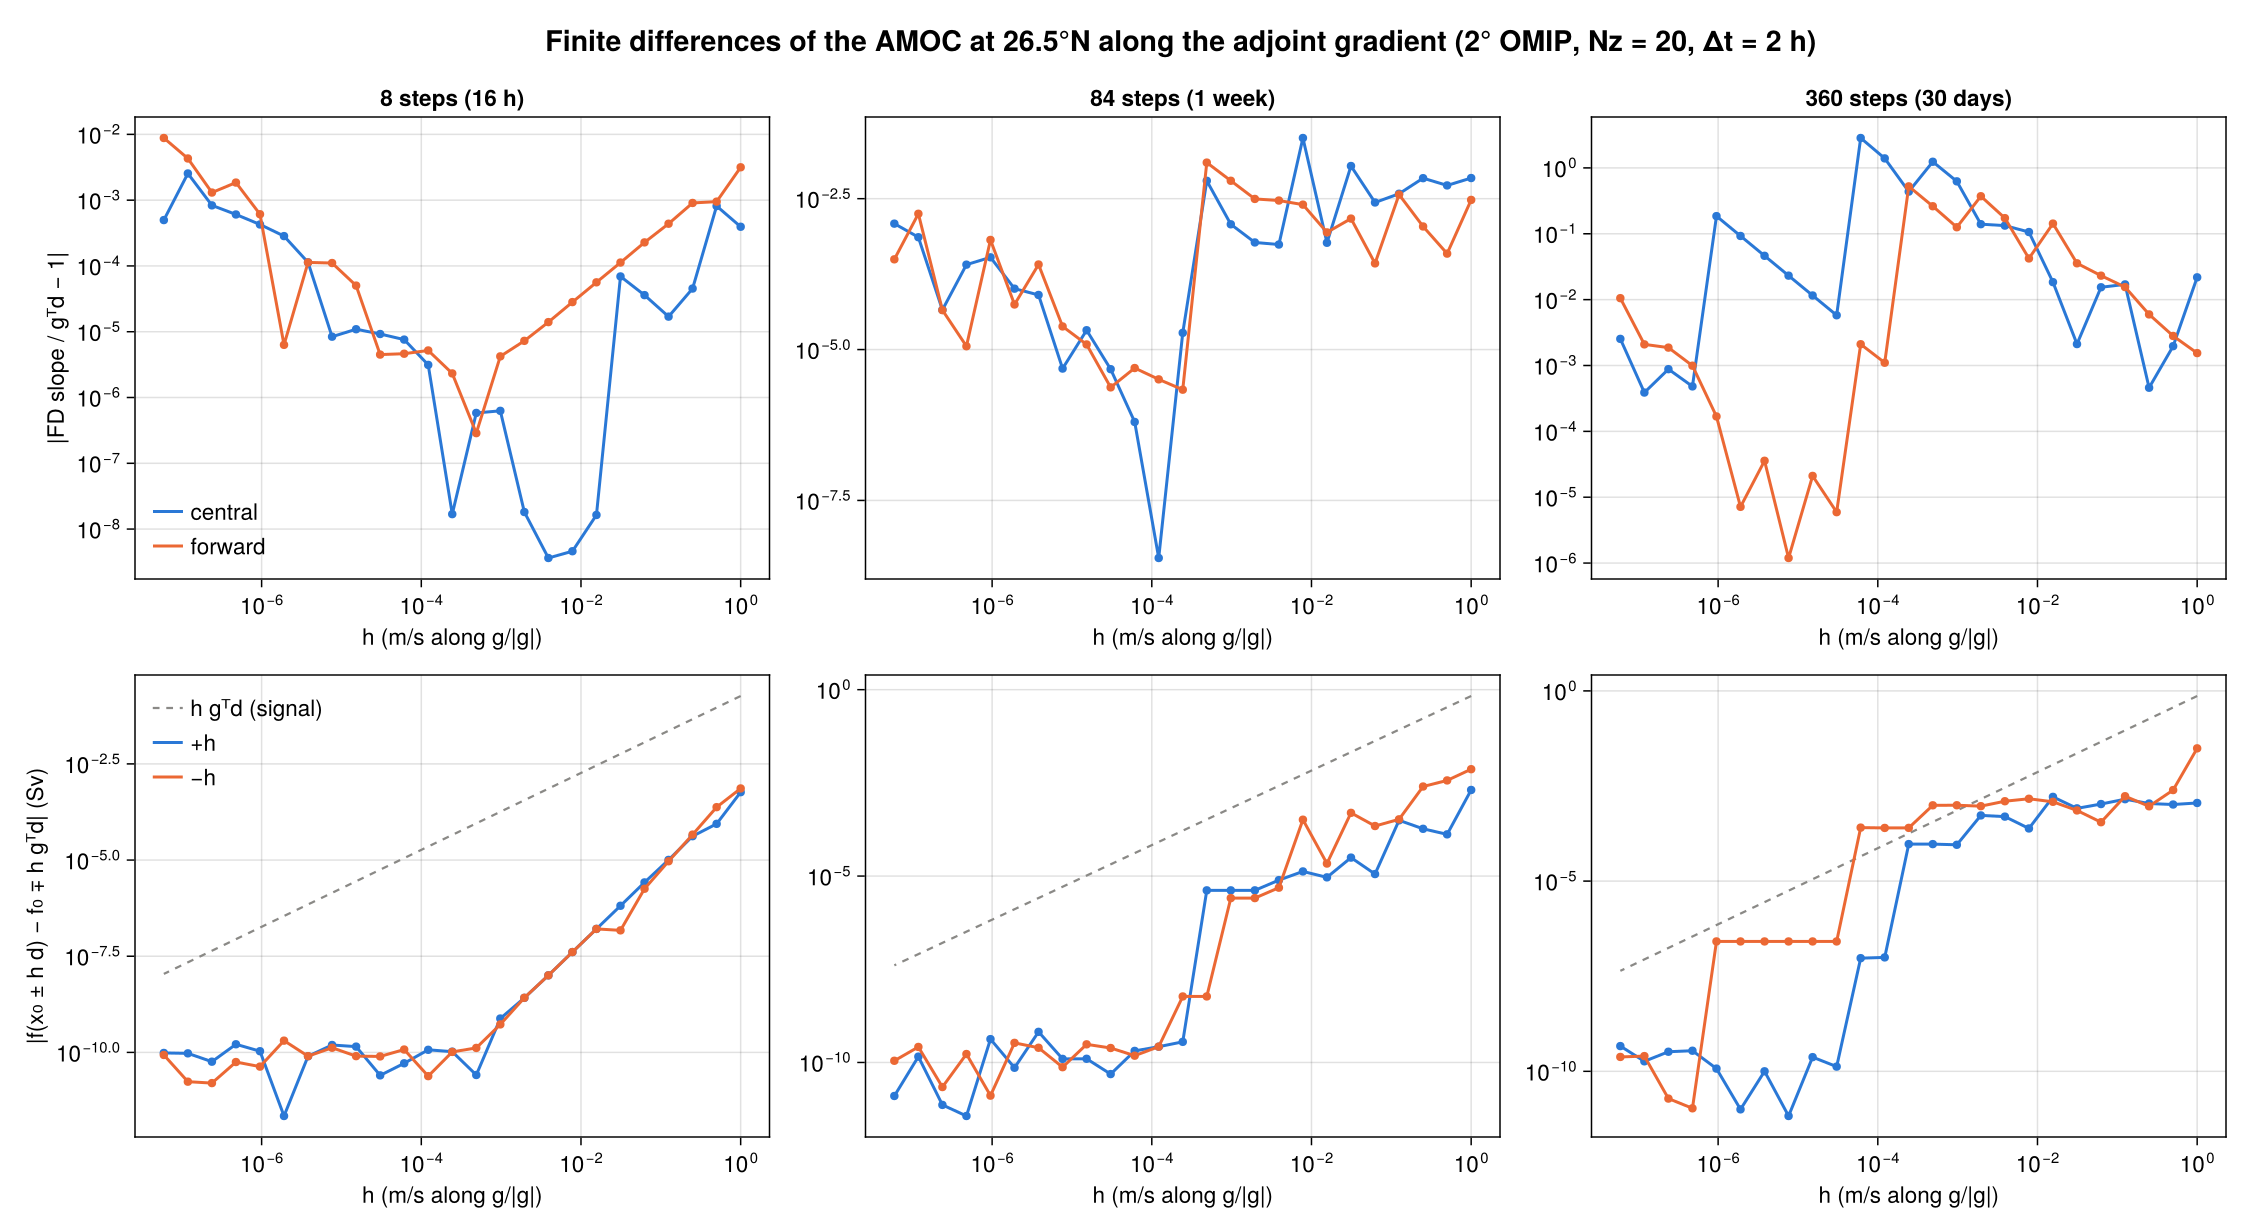
\includegraphics[width=\textwidth]{figures/fd_scans_twodegree_nz20.png}
\caption{Finite-difference scans along the adjoint gradient at 8, 84 and 360 steps. Top: relative
error of the central and forward differences against $\gvec^{\mathsf T}d$. Bottom: residuals of the
linear prediction on each side, with the signal $h\,\gvec^{\mathsf T}d$ dashed. A residual that
plateaus as $h$ shrinks is a jump in $J$.}
\label{fig:fd}
\end{figure}

\section{Results: sensitivity maps}

Figure~\ref{fig:maps} sums $\gvec$ over the forcing slices, which gives the response to a wind
perturbation held over the whole window. It is shown in $4\times4$ blocks of atmosphere cells
(\ang{2.25} boxes). A uniform \SI{1}{m/s} perturbation everywhere changes $J$ by:

\begin{center}\small
\begin{tabular}{@{}rrrrr@{}}
\toprule
Window & $J$ [Sv] & $\sum \partial J/\partial u_{10}$ & $\sum \partial J/\partial v_{10}$ & $\max|\gvec|$ \\
& & [Sv per m/s] & [Sv per m/s] & [Sv per m/s] \\
\midrule
2 steps (4 h) & $-28.56$ & $-0.257$ & $+0.658$ & \num{1.2e-2} \\
8 steps (16 h) & $-11.28$ & $-2.314$ & $-0.715$ & \num{3.0e-2} \\
84 steps (1 week) & $-15.97$ & $-1.583$ & $+0.051$ & \num{2.8e-2} \\
360 steps (30 days) & $+16.63$ & $-0.247$ & $+0.319$ & \num{3.9e-2} \\
\bottomrule
\end{tabular}
\end{center}

\begin{figure}[h]
\centering
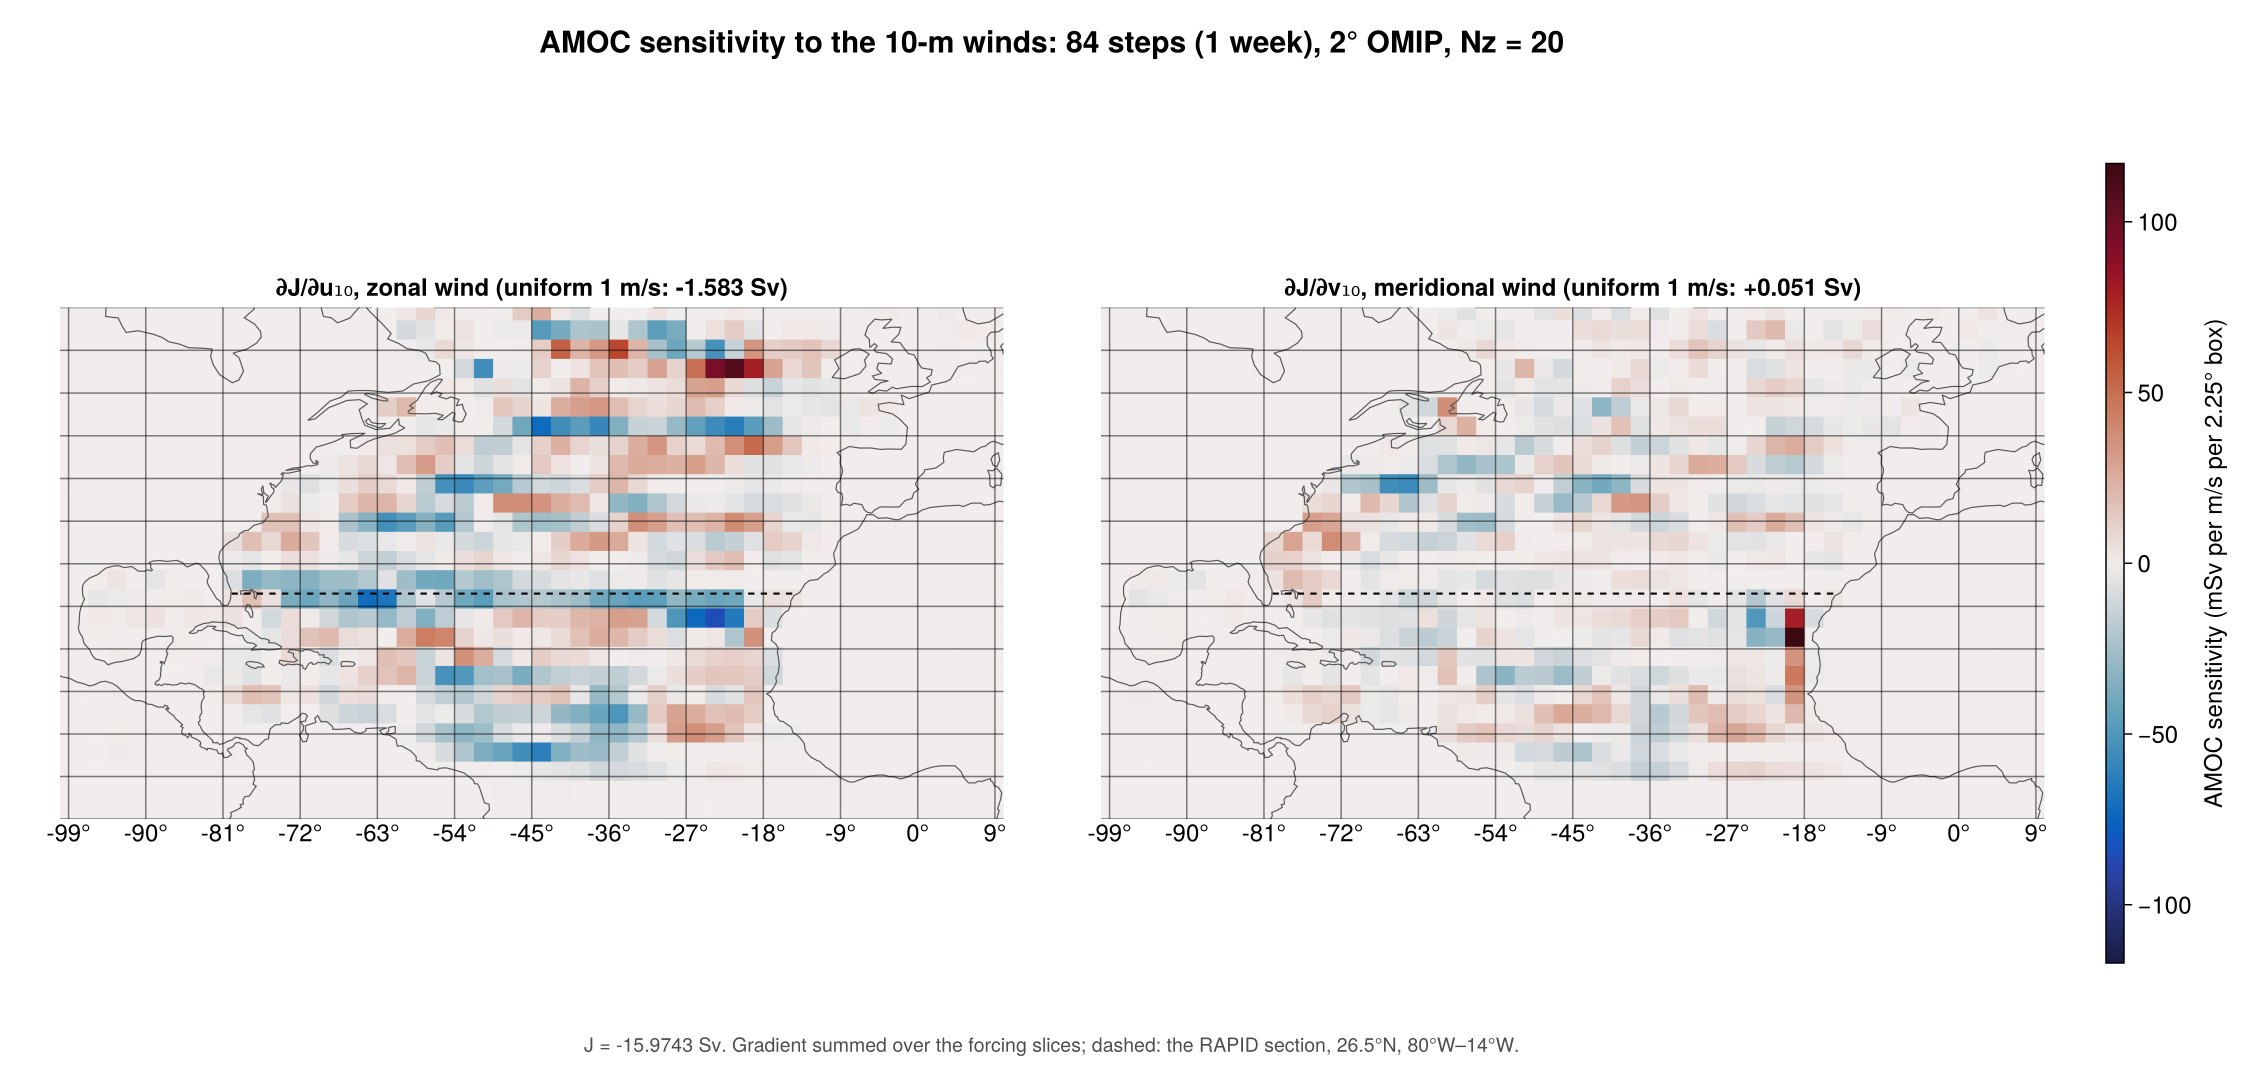
\includegraphics[width=\textwidth]{figures/amoc_sensitivity_twodegree_nz20_84step.png}\\[0.5em]
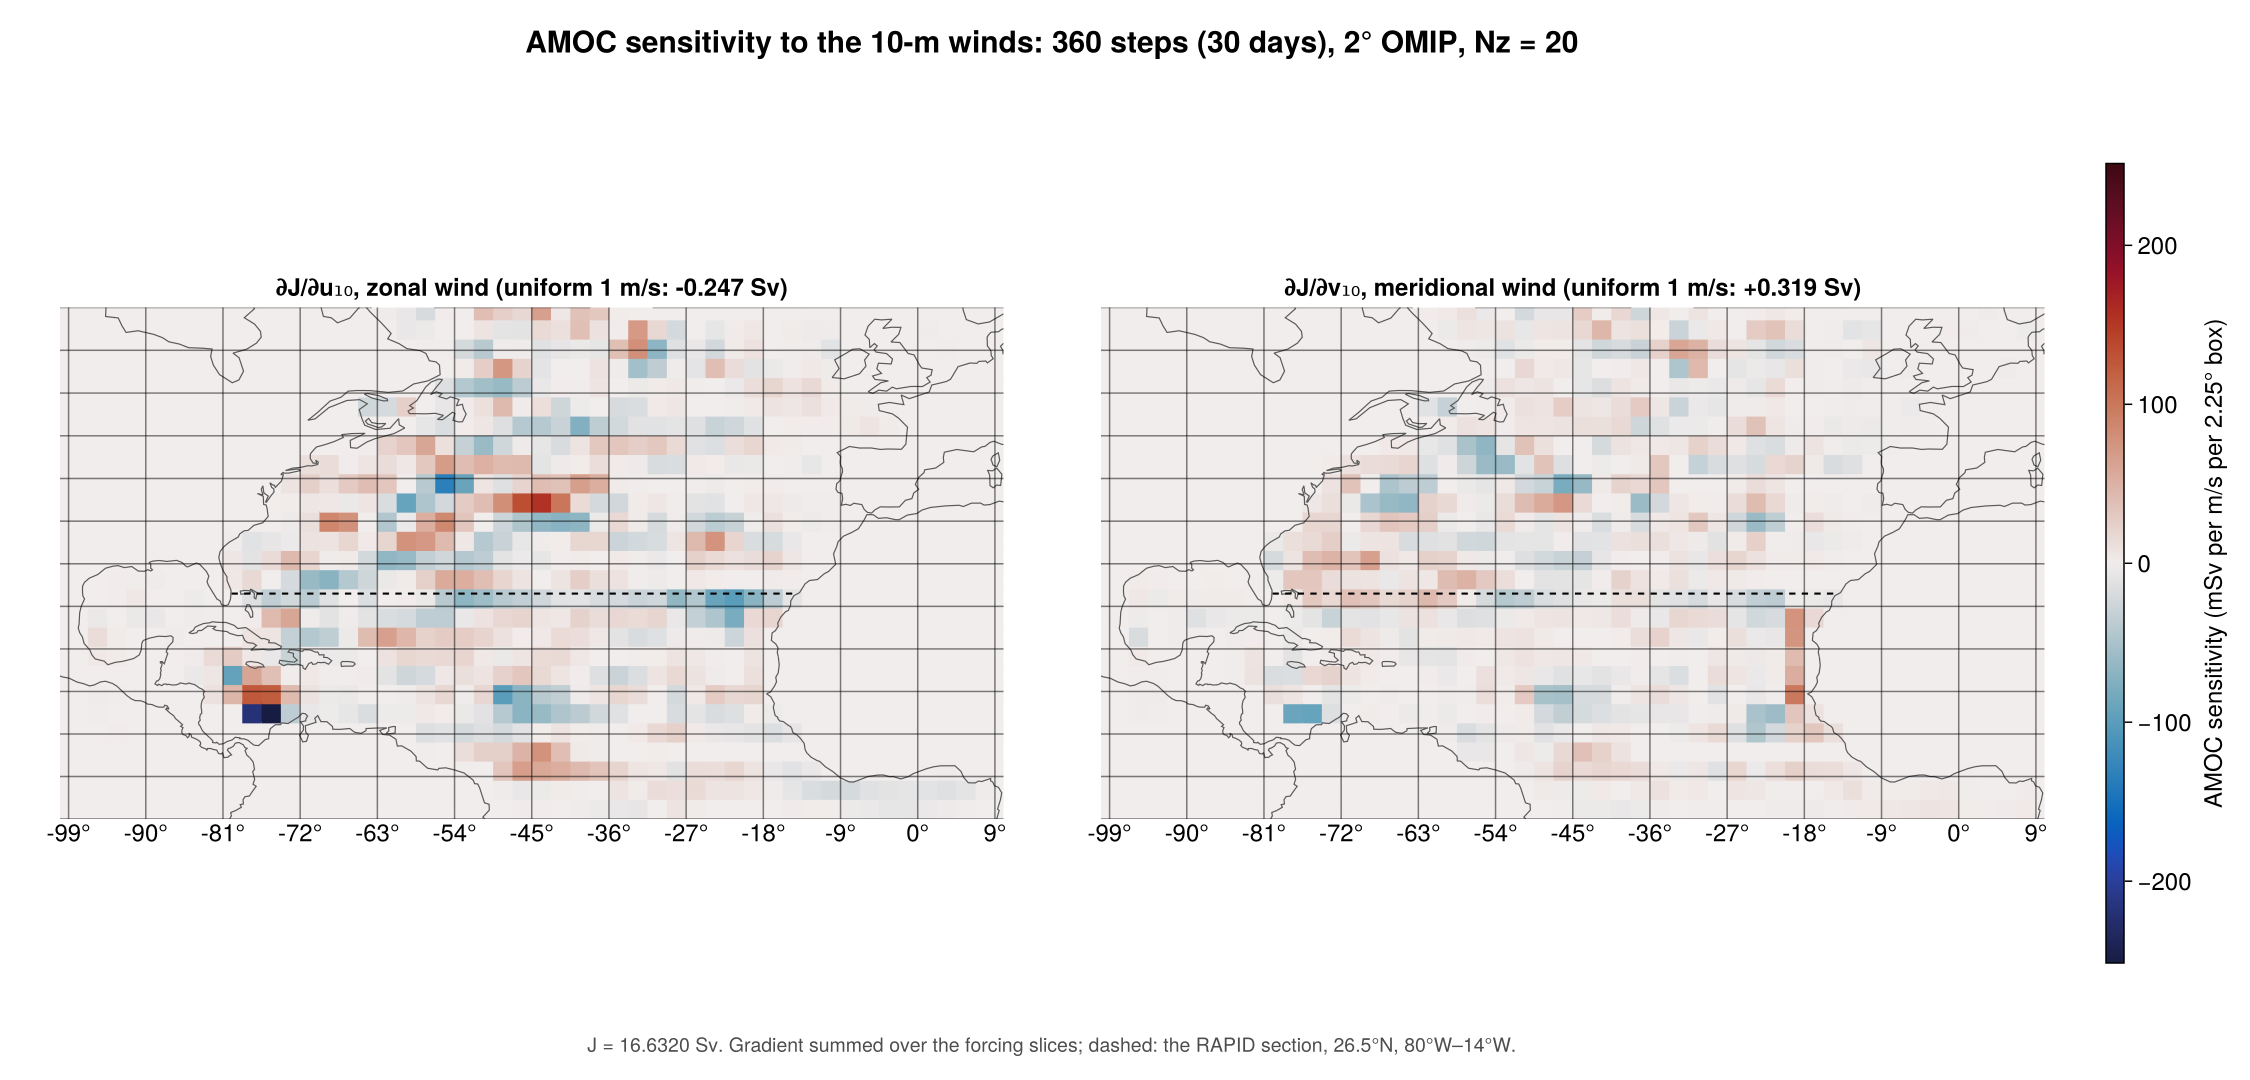
\includegraphics[width=\textwidth]{figures/amoc_sensitivity_twodegree_nz20_360step.png}
\caption{Sensitivity of $J$ to the zonal (left) and meridional (right) \SI{10}{m} wind, summed over
the window, for one week (top) and 30 days (bottom). Dashed: the RAPID section.}
\label{fig:maps}
\end{figure}

After one week, the sensitivity to the zonal wind comes in zonal bands. Along the section and just
south of it, an eastward wind lowers $J$. The meridional-wind sensitivity is concentrated at the
African coast near \ang{18}W, south of the section. After 30 days the pattern breaks up into isolated
boxes, and the largest values lie in the Caribbean (zonal wind near \ang{75}W, \ang{15}N). The
uniform-wind response falls from \SI{-1.6}{Sv} per m/s to \SI{-0.25}{Sv} per m/s, while
$\max|\gvec|$ grows. That is consistent with an objective that, by day 30, depends on where the
transient adjustment has carried the flow more than on the local Ekman response.

\paragraph{Caveat.} These windows start from rest and run through the first month of adjustment.
The adjoint measures the wind-driven response of $\psi$ at \SI{1000}{m} during that transient (Ekman
transport, inertial oscillations, barotropic and baroclinic adjustment), not the buoyancy-driven
overturning. The maps should not be read as an equilibrium sensitivity.

\section{Frozen mixing}
\label{sec:frozen}

Frozen-mixing gradients at 84 and 360 steps (jobs 3572831 and 3572832) use the same windows,
checkpoints and forward model, so $J$ is identical. Table~\ref{tab:frozen} compares them with the full
gradients. The secant slopes are averaged over $h = 1/32$ to \SI{1}{m/s}, where the jumps in $J$ are small
next to $h\,\gvec^{\mathsf T}d$. Along the full gradient's direction, the slope is the central difference
from the FD scans. Along the frozen gradient's direction, it is the forward difference from the frozen
runs' Taylor checks, which carries an $O(h)$ curvature bias.

\begin{table}[h]
\centering\small
\begin{tabular}{@{}lrr@{}}
\toprule
& 84 steps (1 week) & 360 steps (30 days) \\
\midrule
cosine(full, frozen) & \num{0.99964} & \num{0.99418} \\
$\lVert\gvec_{\text{frozen}}\rVert / \lVert\gvec_{\text{full}}\rVert$ & \num{0.9963} & \num{0.9905} \\
\addlinespace
Along $d_{\text{full}}$: FD secant (central) & \num{0.6808} & \num{0.7360} \\
\quad full $\gvec^{\mathsf T}d$ & \num{0.6766} ($-0.6\,\%$) & \num{0.7346} ($-0.2\,\%$) \\
\quad frozen $\gvec^{\mathsf T}d$ & \num{0.6739} ($-1.0\,\%$) & \num{0.7234} ($-1.7\,\%$) \\
\addlinespace
Along $d_{\text{frozen}}$: FD secant (forward) & \num{0.6768} & \num{0.7375} \\
\quad full $\gvec^{\mathsf T}d$ & \num{0.6764} ($-0.1\,\%$) & \num{0.7303} ($-1.0\,\%$) \\
\quad frozen $\gvec^{\mathsf T}d$ & \num{0.6741} ($-0.4\,\%$) & \num{0.7276} ($-1.3\,\%$) \\
\addlinespace
uniform \SI{1}{m/s}: $\sum\partial J/\partial u_{10}$, full / frozen & $-1.583$ / $-1.429$ & $-0.247$ / $-0.234$ \\
uniform \SI{1}{m/s}: $\sum\partial J/\partial v_{10}$, full / frozen & $+0.051$ / $+0.115$ & $+0.319$ / $+0.759$ \\
\addlinespace
gradient compile, first call, repeat call & \SI{29.0}{min}, \SI{2675}{s}, \SI{27}{s} & \SI{30.1}{min}, \SI{2475}{s}, \SI{114}{s} \\
\bottomrule
\end{tabular}
\caption{Full against frozen-mixing gradients. Slopes are in Sv per m/s; the percentages are relative to
the FD secant in the same direction.}
\label{tab:frozen}
\end{table}

Freezing CATKE in the adjoint costs little in direction: the cosine is \num{0.9996} at one week and
\num{0.994} at 30 days. In all four comparisons, however, the full adjoint is the closer predictor of the
finite-amplitude response, and the frozen gradient underpredicts by \SIrange{0.4}{1.7}{\percent}. Freezing
saves no time: compile and repeat call are within \SI{10}{\percent} of the full runs, and the first call
is \SIrange{5}{19}{\percent} longer.
The small change in direction still matters for large-scale patterns. At 30 days, the frozen gradient's
response to a uniform meridional wind is \SI{+0.76}{Sv} per m/s against \SI{+0.32}{Sv} per m/s for the
full gradient, because that sum cancels large values of both signs. The maps differ in the same way
(Figure~\ref{fig:frozen}): the full gradient's largest boxes, in the Caribbean, are absent from the frozen
map, and the frozen map's signal at the African coast is stronger. Which uniform-wind response is right is
a direct finite-difference test along those directions; it has not been run yet.

\begin{figure}[h]
\centering
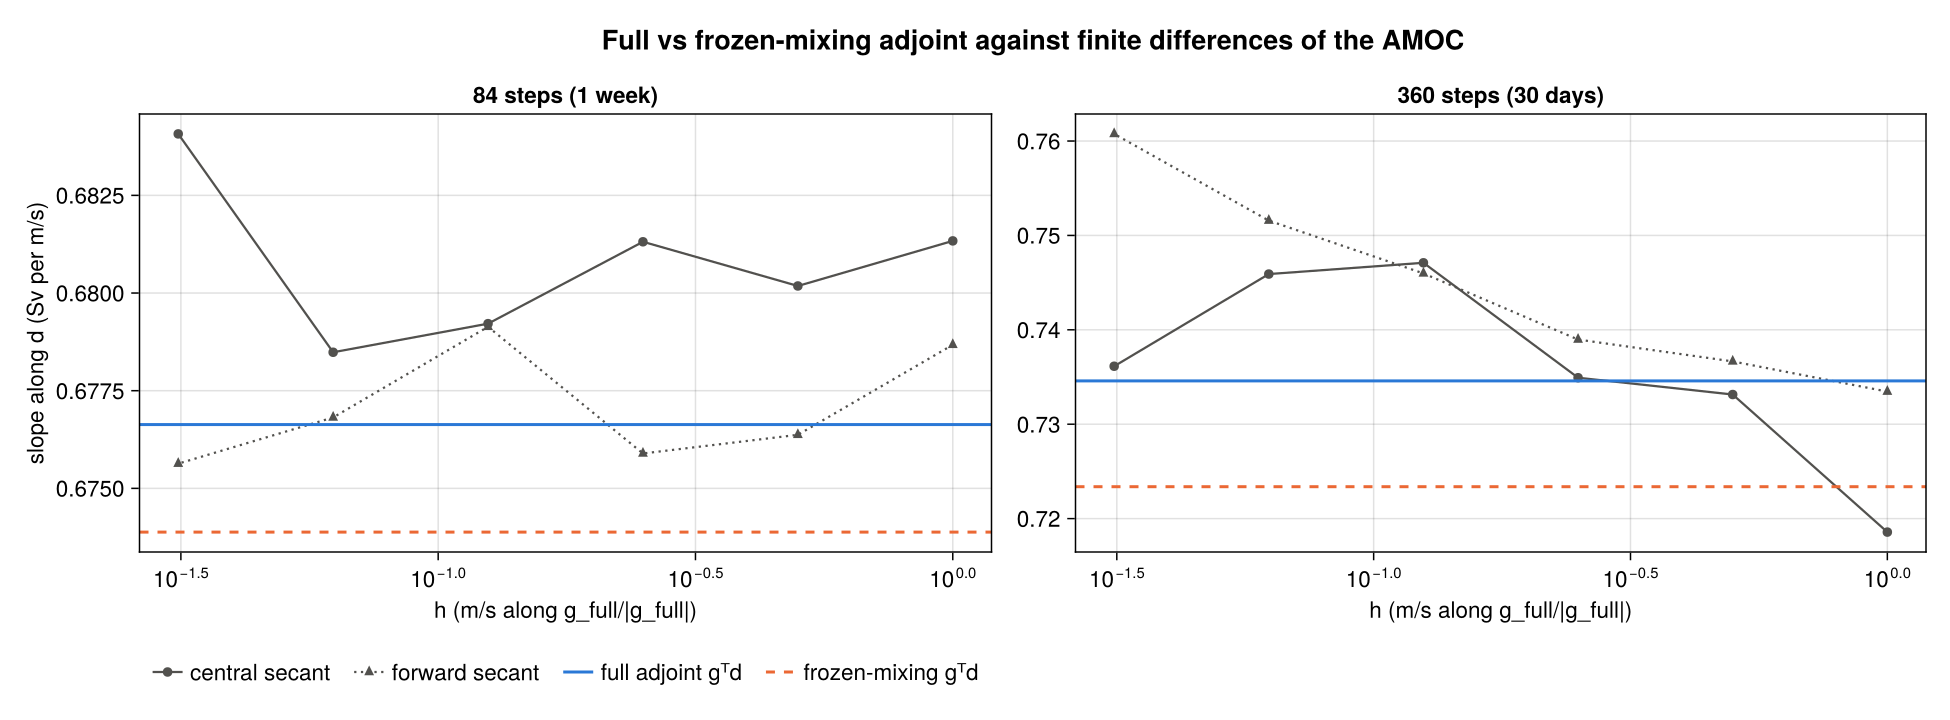
\includegraphics[width=\textwidth]{figures/frozen_vs_full_twodegree_nz20.png}\\[0.5em]
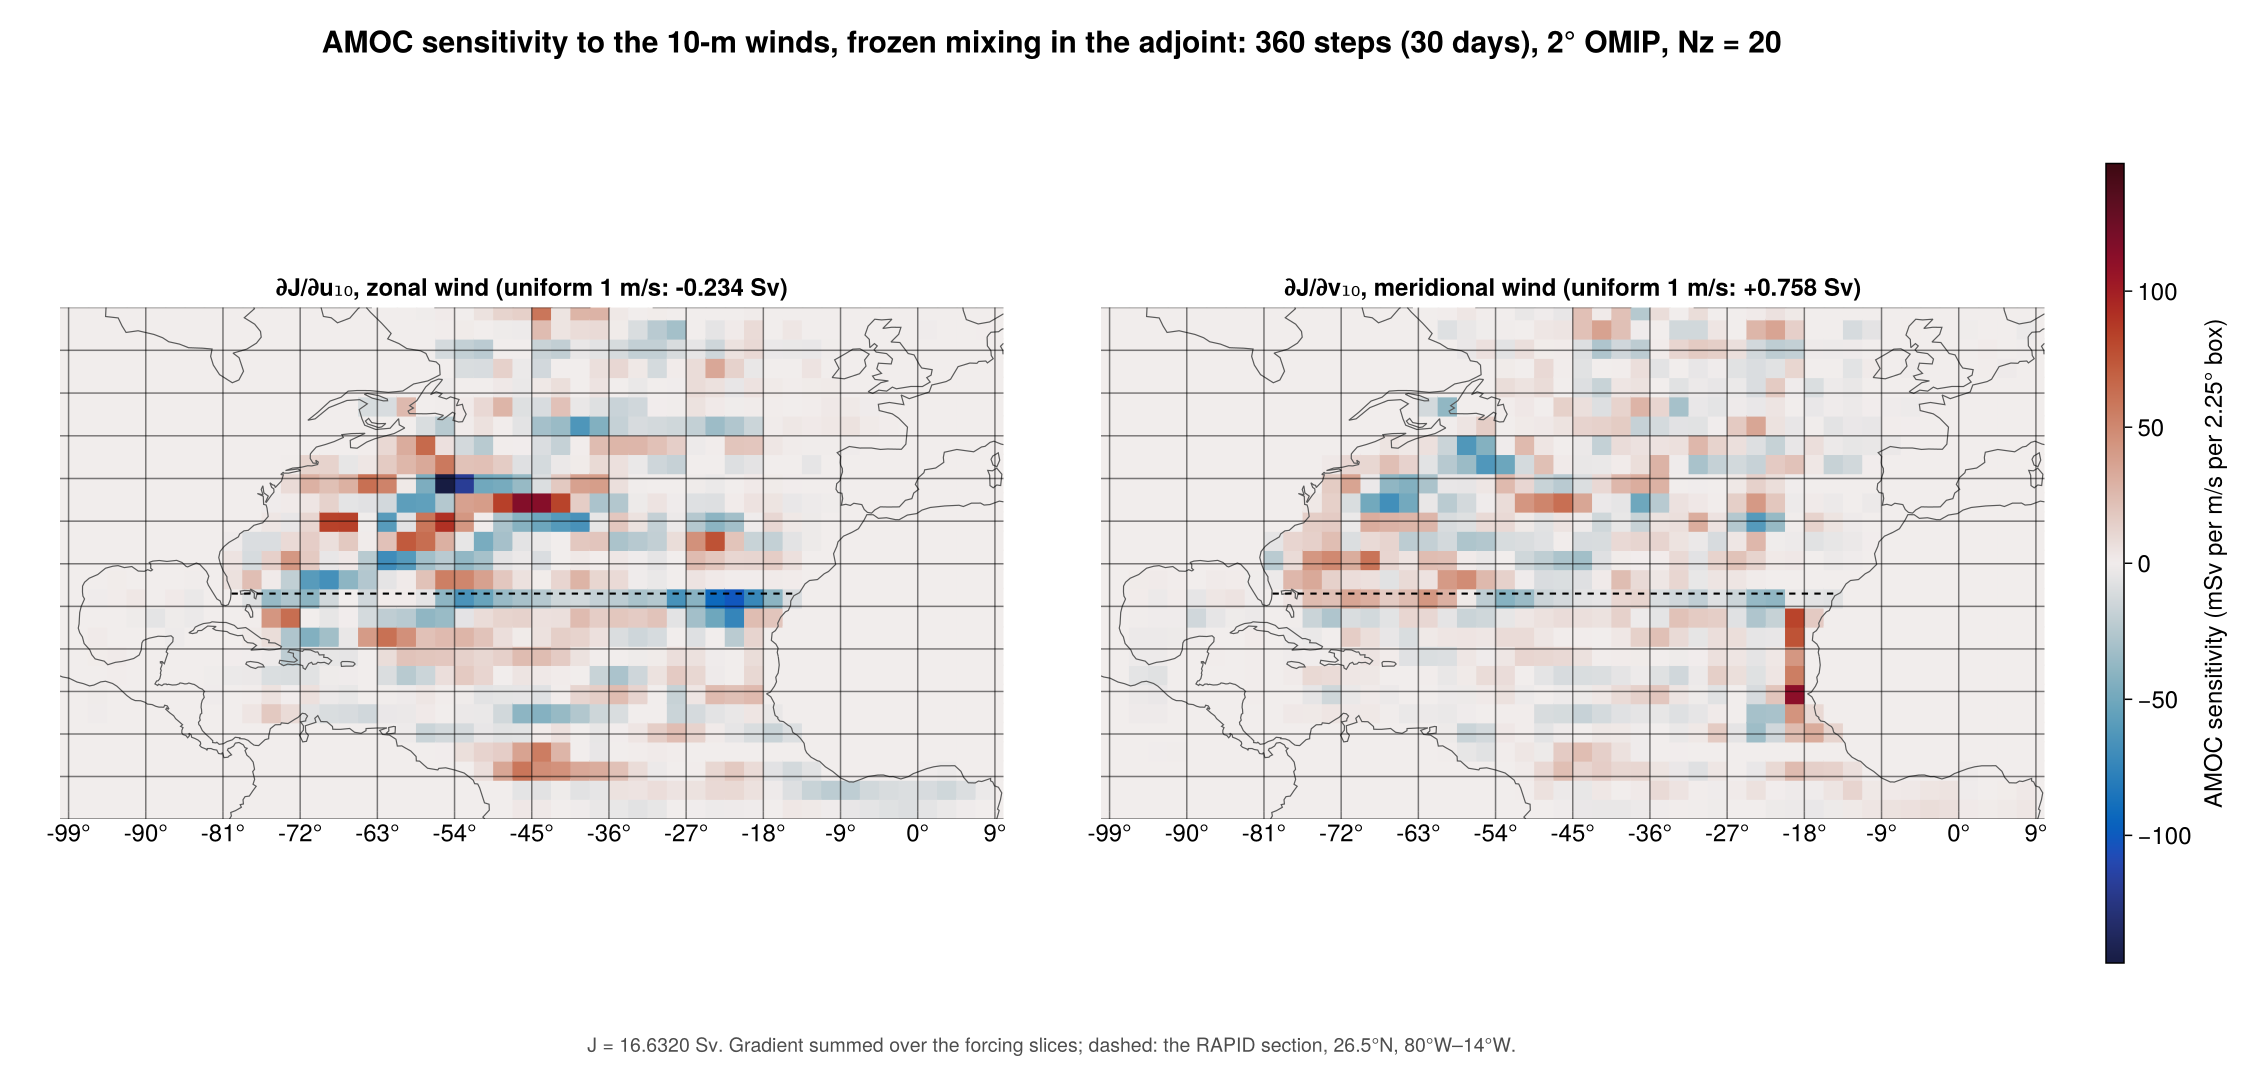
\includegraphics[width=\textwidth]{figures/amoc_sensitivity_twodegree_nz20_360step_frozen.png}
\caption{Top: FD secant slopes along the full gradient's direction, with the full and frozen predictions
there. Bottom: the 30-day frozen-mixing sensitivity map; compare Figure~\ref{fig:maps}, bottom.}
\label{fig:frozen}
\end{figure}

\section{Cost}

\begin{center}\small
\begin{tabular}{@{}rrrrrr@{}}
\toprule
Steps & Checkpoints & Model build & Gradient compile & First call & Repeat call \\
\midrule
2 & 1 & \SI{916}{s} & \SI{27.1}{min} & \SI{2368}{s} & \SI{0.82}{s} \\
8 & 3 & \SI{931}{s} & \SI{28.4}{min} & \SI{2350}{s} & \SI{3.5}{s} \\
84 & 12 & \SI{1022}{s} & \SI{27.3}{min} & \SI{2241}{s} & \SI{28}{s} \\
360 & 30 & \SI{1423}{s} & \SI{29.1}{min} & \SI{2367}{s} & \SI{104}{s} \\
\bottomrule
\end{tabular}
\end{center}

Compile and first call do not depend on the window length. Differentiating the whole window as one
module took \SI{47.8}{min} to compile at only 2 steps, and the cost grows with $N$; a rolled window does
not fit in memory, because Enzyme's reverse loop carries \SI{73}{GiB} of zero shadow state. The first
call's \SI{\sim 39}{min} is host-side: XLA logs nothing during it. It is most likely Julia compiling the
five compiled functions' call wrappers for the model type (\SI{753}{s} for the smaller ECCO4 model).

\section{Next runs}
\label{sec:next}

All settings come from JSON files in \path{adjoint/configs/}. The driver is
\path{adjoint/test_omip_adjoint.jl}, and its stages (\texttt{cpu}, \texttt{primal},
\texttt{gradient}, \texttt{fd\_scan}) are chosen by the \texttt{stages} key.

The results files grow to hundreds of MB at long windows. They are reduced on a Lonestar6 CPU node, and
only the summary is copied back and plotted locally:
\begin{verbatim}
SCRIPT=adjoint/reduce_gradients.jl \
  CONFIG=adjoint/configs/reduce_twodegree_nz20.json \
  sbatch -J ReduceGrad adjoint/omip_cpu.slurm
julia +1.12 --project=adjoint/plots adjoint/plot_amoc_sensitivity.jl \
  adjoint/configs/plot_twodegree_nz20_360step_checkpointed.json
\end{verbatim}
Next:
\begin{enumerate}
\item Finite differences along the uniform zonal and meridional winds at 30 days. These decide between the
      full and frozen uniform-wind responses (\SI{+0.32}{Sv} against \SI{+0.76}{Sv} per m/s for $v_{10}$),
      and they test the gradient along a physically meaningful direction rather than its own.
\item Merge upstream \texttt{ss/omip-prototype} again, including \texttt{c6eede8f} (a fold-halo patch
      and a \texttt{restore\_prognostic\_state!} override), and repeat the 2-step verification. An
      earlier merge without that commit broke the package and was reverted.
\item Longer windows. The in-memory forcing and its shadow grow with the window. By estimate, nine
      Float64 fields on $640\times320$ are \SI{14.7}{MB} per slice, or \SI{3.7}{GB} for 30 days; doubled
      by the shadow, that is \SI{7.3}{GB}. A year would need \SI{86}{GB}, more than one A100 holds. A year
      therefore needs the forcing streamed per checkpoint segment, a coarser control (for example daily
      or monthly winds), or the ECCO4 monthly forcing.
\item Nz = 70, and a spun-up initial state instead of rest.
\end{enumerate}

A gradient job is submitted from \path{experiments/OMIPSimulations} on Lonestar6 with:
\begin{verbatim}
CONFIG=adjoint/configs/twodegree_nz20_360step_checkpointed.json \
  sbatch -J Grad360Ckpt -p gpu-a100-dev -t 02:00:00 adjoint/omip_adjoint.slurm
\end{verbatim}
The gradient runs only on Lonestar6's x86\_64 A100 nodes. On Vista's aarch64 nodes, LLVM fails in the
first call with ``fixup value out of range''.

\end{document}
